\question ICMP报文的传输方式是
\par\fourch{无连接的UDP数据报形式传送}{面向连接的TCP报文形式传送}{放在IP数据报的首部字段中传送}{\textcolor{red}{放在IP数据报的数据字段中传送}}
\begin{solution}网际报文控制协议(ICMP)属于IP层协议。ICMP报文作为IP层数据报的数据,加上IP数据报的首部,组成IP数据报发送出去。
\end{solution}
\question 当路由器无法转发或传送IP数据报时,向初始源站点发回一个( )报文
\par\twoch{路由重定向}{\textcolor{red}{目标站不可到达}}{源抑制}{子网掩码请求}
\begin{solution}当路由器无法转发或者传送IP数据报时,向初始源点发回一个目的站不可达报文。目的站不可达报文的代码字段包含了进一步描述问题的整数,以表明不可达的原因,如端口不可达、目的网络未知、目的主机未知等。
\end{solution}
\question (北京理工大学,2005年)Internet的网络层有4个重要的协议,分别是
\par\fourch{IP,ICMP,ARP,UDP}{TCP,ICMP,UDP,ARP}{\textcolor{red}{IP,ICMP,ARP,RARP}}{UDP,IP,ICMP,RARP}
\begin{solution}解题技巧:ICMP四个选项都有,而IP是网络层的,ARP和RARP都是和IP转换相关,所以这3个肯定同时存在,故答案选C。UDP和TCP是传输层协议。
\end{solution}
\question 在TCP/IP体系结构中,直接为ICMP提供服务的协议是( )
\par\twoch{PPP}{\textcolor{red}{IP}}{UDP}{TCP}
\begin{solution}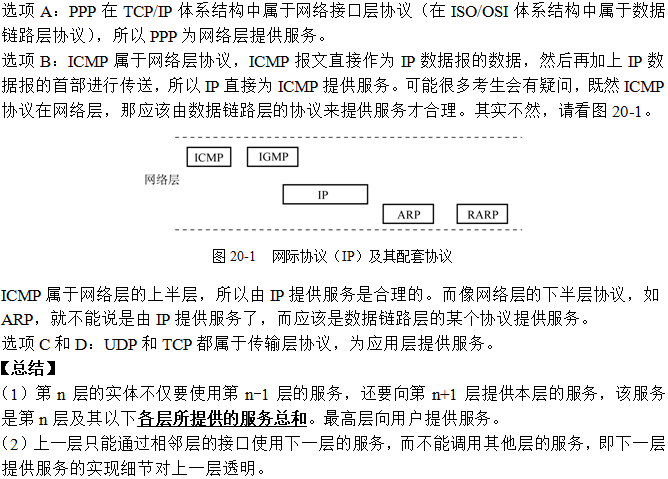
\includegraphics[width=3.46875in,height=2.48958in]{computerassets/1A93DAF555282F20061DC42F39C4EF55.png}
\end{solution}
